\appendix
\titleformat{\chapter}[block]{\normalfont\LARGE\bfseries}{Appendix \thechapter \;\textendash\;}{0ex}{\vspace{-4cm}}[\vspace{4.5cm}]
\titlespacing{\chapter}{0cm}{0cm}{0cm}

\chapter{Various Parameters}
\label{chap:appendix}

\begin{figure}[H]
  \centering
  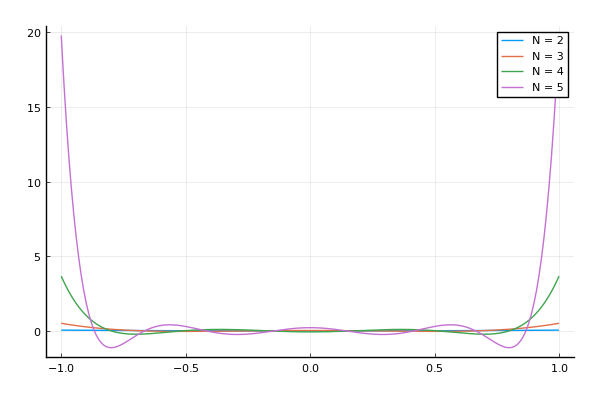
\includegraphics[width=0.6\linewidth]{results/bump/solution-increasing-order}
  \caption[Bump parameter solutions]{Solutions with bump parameters.}
  \label{fig:bump-solutions}
\end{figure}

\begin{figure}[H]
  \centering
  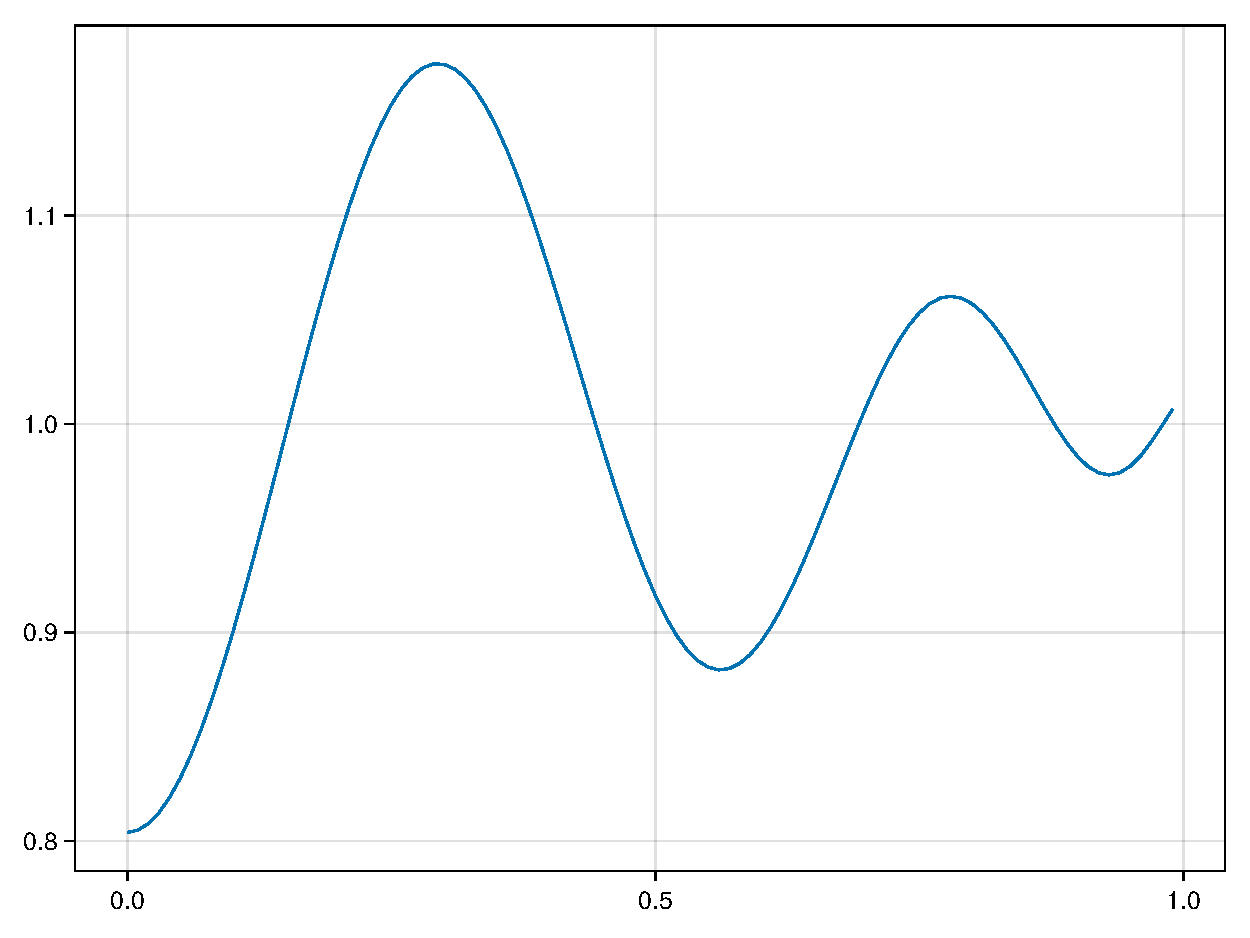
\includegraphics[width=0.7\linewidth]{results/attrep/energy-dependence-on-r.pdf}
  \caption[Spatial energy dependence on $r$]{Plot of the spatial energy dependence on $r$, for different values of the domain support radius $R$. As one can see, $\tilde{E}(\vec{x}) = \jacobivec{x} Q_{\alpha,\beta} \vec{\rho}$ constant and this figure is only present as visual proof to increase our confidence in the construction of the spectral method.}
  \label{fig:spatial-energy-dependence}
\end{figure}

\pagebreak
\begin{figure}[H]
  \centering
  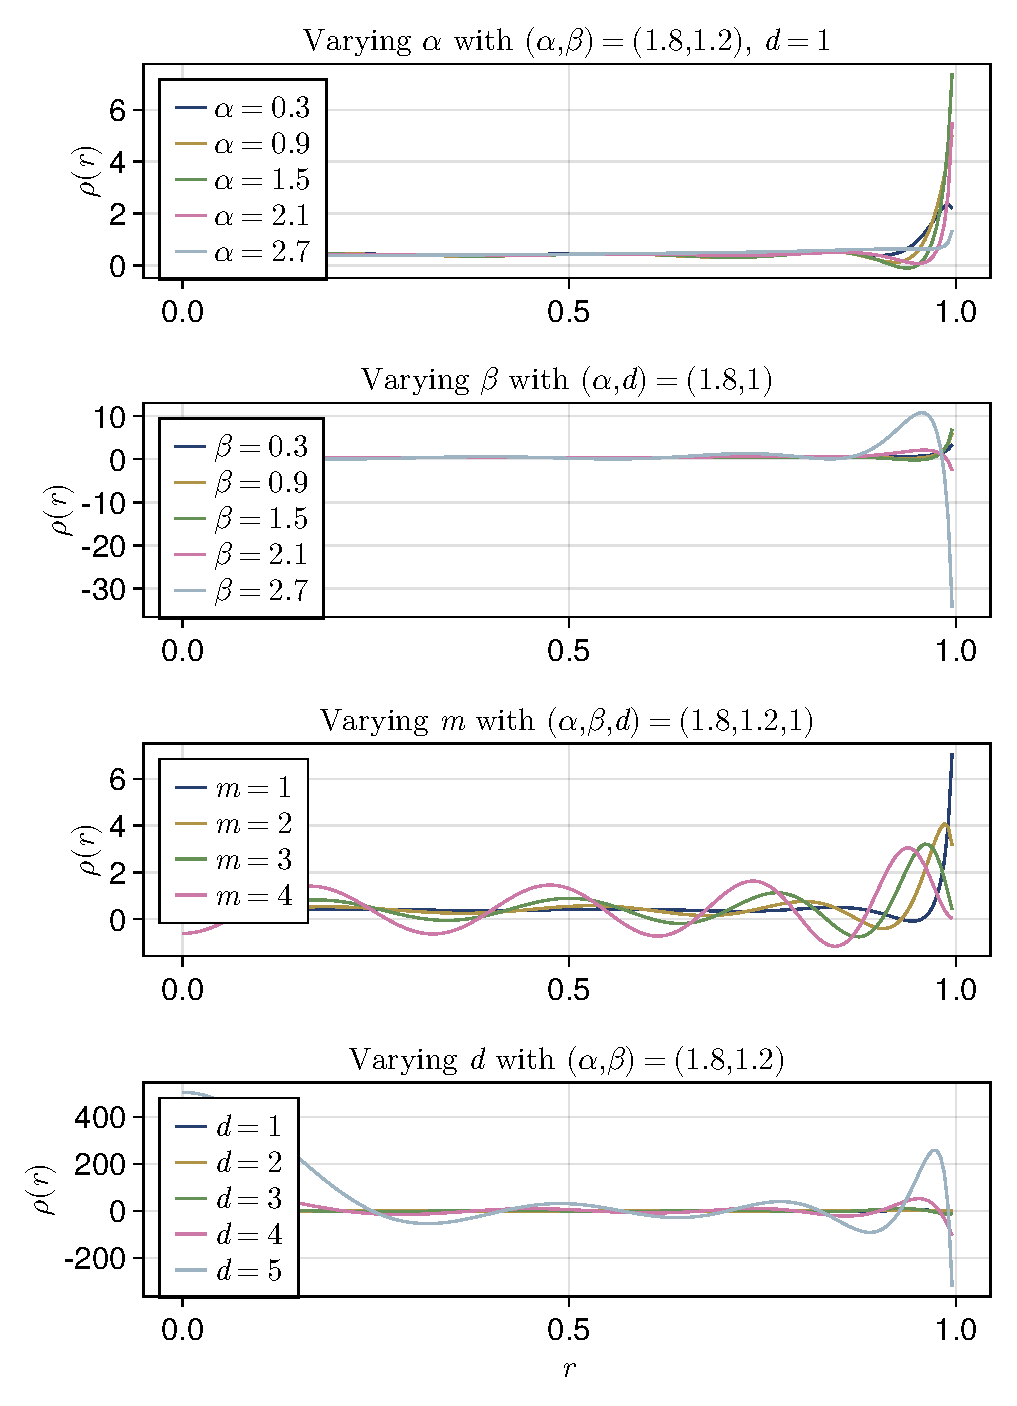
\includegraphics[width=0.9\linewidth]{results/attrep/varying-parameters.pdf}
  \caption[Varying parameters in the solver]{
    Varying different parameters in the solver to demonstrate their effect.
    See also, \Cref{fig:varying-R-solutions}.
  }
  \label{fig:varying-parameters}
\end{figure}
\pagebreak

% \chapter{Supplemental Proofs}

\chapter{Code Snippets}
\label{appendix:code-snippets}
\begin{minted}{cpp}
void ParticleBox::simulate(size_t timesteps) {
  double afterAccelerations[PARTICLES][DIMENSION];
  f(afterAccelerations);
  for (size_t t = 0; t < timesteps; t++) {
    ParticleVectors beforeAccelerations = afterAccelerations;
    memcpy(beforeAccelerations, afterAccelerations, PARTICLES * DIMENSION * sizeof(double));
    for (size_t i = 0; i < PARTICLES; i++) {
      for (size_t d = 0; d < DIMENSION; d++)
        positions[i][d] += p.tau * velocities[i][d] + square(p.tau) / 2 * beforeAccelerations[i][d];
    }

    f(afterAccelerations);
    for (size_t i = 0; i < PARTICLES; i++) {
      for (size_t d = 0; d < DIMENSION; d++) {
        velocities[i][d] += (p.tau / 2 * (beforeAccelerations[i][d] + afterAccelerations[i][d])) / p.boxScaling;
      }
    }
    reflectParticles();
  }
}
\end{minted}
